\documentclass[english,a4paper,11pt]{report}
\usepackage[utf8]{inputenc}
\usepackage[T1]{fontenc}
\PassOptionsToPackage{english}{babel}
\usepackage{graphicx}
\usepackage{fullpage}
\usepackage{eso-pic}
\usepackage{cite}
\usepackage{wrapfig}
\usepackage{url}
\usepackage[english]{babel}
\usepackage{fancyhdr}
\usepackage{hyperref}
\usepackage[lastpage,user]{zref}
\usepackage{amsmath}
\usepackage{amssymb}
\usepackage{listings}
\usepackage{array}

\cfoot{\thepage\ of \zpageref{LastPage}}
\pagestyle{fancy}
\usepackage[headsep=1cm,headheight=61pt,footskip=3cm]{geometry}


\newcommand{\HRule}{\rule{\linewidth}{0.5mm}}
 \newcommand{\ts}{\textsuperscript}
\newcommand{\blap}[1]{\vbox to 0pt{#1\vss}}
\newcommand\AtUpperLeftCorner[3]{%
  \put(\LenToUnit{#1},\LenToUnit{\dimexpr\paperheight-#2}){\blap{#3}}%
}
\newcommand\AtUpperRightCorner[3]{%
  \put(\LenToUnit{\dimexpr\paperwidth-#1},\LenToUnit{\dimexpr\paperheight-#2}){\blap{\llap{#3}}}%
}
\newcommand\AtLowerRightCorner[3]{%
  \put(\LenToUnit{\dimexpr\paperwidth-#1},\LenToUnit{#2}){#3}%
}
 
\title{\LARGE{Automation and robotic project 1}}
\author{\textsc{Breton-Belz} Emmanuel - UNISA 2015 - 2016}
\date{\today}
\makeatletter

\renewcommand{\headrulewidth}{1pt}
\fancyhead[C]{\@author} 
\fancyhead[L]{\leftmark}
\fancyhead[R]{
\includegraphics[width=2cm]{images_not_compressed/unisaLogo.jpg}}
\addto\captionsenglish{
  \renewcommand{\contentsname}
    {Table of contents}
}
\renewcommand{\footrulewidth}{1pt}
\fancyfoot[R]{\leftmark}
		 
\begin{document}
	%\setcounter{tocdepth}{4}
	
	\begin{titlepage}
	\begin{center}
	        \vspace*{6cm}
	        \textsc{\@title}
	        \HRule
	        \vspace*{0.5cm}
	        \large{\@author} 
	 \end{center}
	 
	
	    \AddToShipoutPicture{%
	      \AtUpperLeftCorner{1.5cm}{1cm}{
\includegraphics[width=4cm]{images_not_compressed/unisaLogo.jpg}}
	     }
	     
	\begin{center}
		\vspace*{2.5cm}
		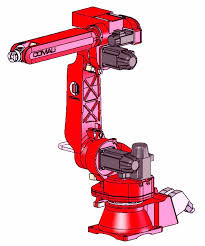
\includegraphics[width=8cm]{images_not_compressed/smart5.jpg}
	\end{center}
	 

	
	\end{titlepage}
	\ClearShipoutPicture
	
	\tableofcontents

	\chapter{Introduction}
		
	In this project we apply the theory seen in automatic and robotic course.
	The aim is creating a function that returns the most important parameters for moving the end-effector of the robot. We can see it on the figure \ref{endEf} with it\rq{}s own axes \lq\lq{}ANS\rq\rq{}. This parameters are the position and the orientation of the end-effector, the rotation matrix of the end-effector and the roto-translation matrices for the differents input parameters (angles and translations of the joints).
	
	The function takes two parameters, the first is a vector values reprensenting the translation or the rotation of each axe. The is the type of representation we are in. It can be \lq\lq{}ZYZ\rq\rq{} or \lq\lq{}RPY\rq\rq{} (roll, pitch, yaw).
	\begin{figure}[h]
	\center
		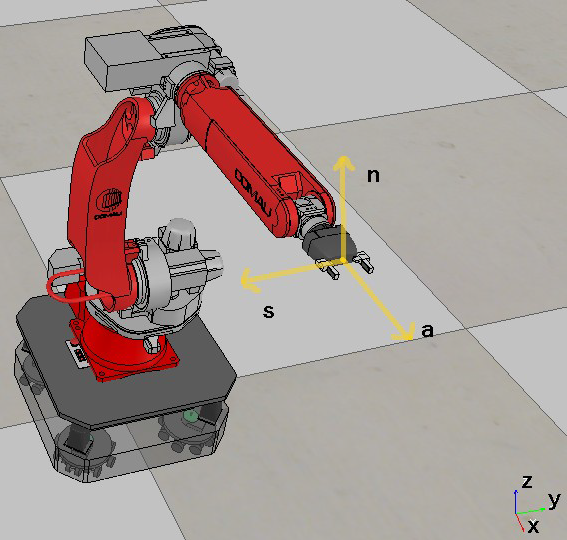
\includegraphics[width=9cm]{images_not_compressed/endEffector.png}
		\label{endEf}
		\caption{Robot smart5 six with a pince on the end-effector}
	\end{figure}

	\chapter{Work}
	\section{Compute the roto-translation matrix}
	\subsection{Required}
	
	
	
	
	\begin{wrapfigure}{r}{0.4\textwidth} 
		\vspace{-1cm}

 		 \begin{center}
  			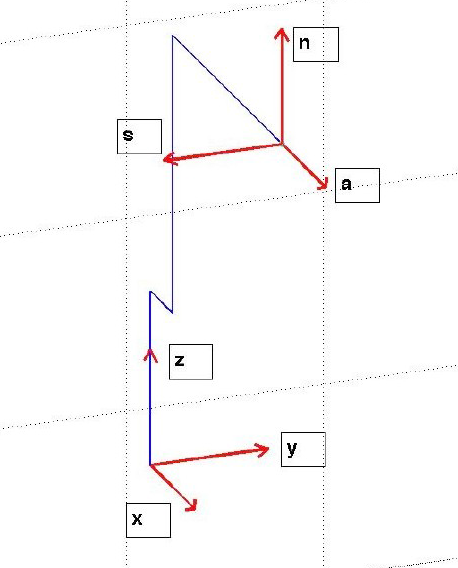
\includegraphics[width=7cm]{images_not_compressed/alphaAngles.png}
			\label{alpha}
			\caption{Stick view of the Smart5 Six}
 		 \end{center}
	\end{wrapfigure} 
	
	\vspace{1cm}
	
	To get the roto-translation matrix we need to multiply the different matrices for each junction and the $A^{b}_{0}$ and $A^{n}_{e}$ which are two constant matrix respectly represent the b to 0 transformation matrix and the n to e transformation matrix.\\
	We also need the $\alpha$ angles for each junction. We put them in a vector called alpha\_i which is $\begin{bmatrix}\frac{\pi}{2} & \frac{\pi}{2} & \frac{-\pi}{2} & 0 & \frac{-\pi}{2} & \frac{\pi}{2} & \frac{-\pi}{2} & 0\end{bmatrix}$. We obtain this values by comparing the junction $i$\rq{}s Z axis with the $(i-1)$\rq{}s Z axis.\\
	On the figure \ref{alpha} we can see the different axes of the robot. Each line correspond to a axe and the $Z$ vector corresponds to the rotation axe. Then, if we take the second line, we have to make a clockwise rotation of $\frac{\pi}{2}$ to get its $Z$ axe.\\
	We also need a vector that we will call $a$ that stores the distances between the axes that have the same $Z$ orientation 2 by 2. We get this values in on the figure 4 of the documentation of the project. With the same figure we fill the $di$ vector which stores the distance of the axes that doesn\rq{}t have the same $Z$ orientation.
	Finally, we create the $teta\_i$ vector to store the angles of in parameter of the function.

	\begin{figure}
	\centering
		\begin{tabular}{c|c|c|c|c|c}
		Link & $\alpha$ & $\theta$ & a & d & $ \overline{q}$\\
		\hline
		1 & $\frac{\pi}{2}$ & 0 & 0 & $d_1$ &$ d_1$\\
		\hline
		2 & $\frac{\pi}{2}$ & 0 & 0 & $d_2$ & $d_2$\\
		\hline
		3 & $\frac{-\pi}{2}$ & $\theta_3$ & 0.15 & 0.45 & $\theta_3$\\
		\hline
		4 & 0 & $\theta_4$ & 0.59 & 0 & $\theta_4$\\
		\hline
		5 & $\frac{-\pi}{2}$ & $\theta_5$ & 0.13 & 0 & $\theta_5$ \\
		\hline
		6 & $\frac{\pi}{2}$ & $\theta_6$ & 0 & 0.64707 & $\theta_6$\\
		\hline
		7 & $\frac{-\pi}{2}$ & $\theta_7$ & 0 & 0 & $\theta_7$ \\
		\hline
		8 & 0 & $\theta_8$ & 0 & 0.095 & $\theta_8$\\
		\end{tabular}
		\caption{DH parameter table for each junction}
	\end{figure}

	
	
	\subsection{Compute the matrix}
	We learned during the lessons that :
	$A^{i-1}_{i}(q_{i}) = A^{i-1}_{i\rq{}}A^{i\rq{}}_{i} = 
	\begin{bmatrix} 
	c_{\theta_{i}} & - s_{\theta_{i}} c_{\alpha_{i}} & s_{\theta_{i}} s_{\alpha_{i}} & a_{i} c_{\theta_{i}}\\
	s_{\theta_{i}} &  c_{\theta_{i}} c_{\alpha_{i}} & -c_{\theta_{i}} s_{\alpha_{i}} & a_{i} s_{\theta_{i}}\\
	0 &  s_{\alpha_{i}}  & c_{\alpha_{i}} & d_{i}\\
	0 & 0 & 0 & 1
	\end{bmatrix} $

	To store efficently the values, we use a tridimentionnal matrix $4\times4\times8$ which makes a $4\times4$ per each junction. Using a for loop, we fill the matrix using the values of the $a$, $di$ and $teta\_i$ vectors.
	
	\subsection{Get the position and the rotation matrix relative to the end-effector}
	
	To get the position of the end-effector and the rotation matrix, we have to compute the general transition matrix denoted $T$. The formula is : $A^b_0\times\prod_{i=1}^n A^{n-1}_n\times A^n_e$.
	It corresponds to the $A^b_e(\overline{q})$ which is equals to 
	$\begin{bmatrix} 
	R^b_e(\overline{q}) & O^b_e(\overline{q})\\
	\overline{O}^T & 1
	\end{bmatrix} $
	It last to extract the $R^b_e(\overline{q})$ and the $O^b_e(\overline{q})$ matrices of the $A^b_e(\overline{q})$ matrix by writing :
	\begin{lstlisting}
	p = T([1 2 3], 4);
	R = T([1 2 3], [1 2 3]);
	 \end{lstlisting}
	 
	 There we have the $A$ transition matrix of all the junctions, the matrix of rotation from the base to the end-effector and the position of the end-effector. Now we will focus on the the Euler angles.
	 
	 
	 \section{Get the Euler angles}
	\subsection{Divide the different referentials}
		The two different referentials are \lq{}ZYZ\rq{} and \lq{}RPZ\rq{}. They are not axed the same way, that is why we differenciate 2 cases to extract the Euler angles $\phi$, $\theta$ and $\psi$.
		
	\subsection{Extraction of the angles}
	In \lq{}ZYZ\rq{} we have :
	\begin{lstlisting}
	phi = atan2(R(2,3),R(1,3));
	theta = atan2(sqrt(R(1,3)^2 + R(2,3)^2), R(3,3));
        psi = atan2(R(3,2), -R(3,1));
	\end{lstlisting}	
	
	and for \lq{}RPY\rq{} referential we need :
	\begin{lstlisting}
	phi = atan2(R(2,1),R(1,1)); 
	theta = atan2(-R(3,1), sqrt(R(3,2)^2 + R(3,3)^2));
	psi = atan2(R(3,2), -R(3,3));
	\end{lstlisting}
	
	There we compute the Euler angles in the good referential.

	\listoffigures
	
\end{document}